\section*{25. Квазитранзитивные и ациклические отношения. Свойства и примеры.}
\par Пусть на множестве M задано отношение $\preccurlyeq$. По нему можно построить строгое отношение $\prec$ по правилу: $x \prec y$, если $x \preccurlyeq y$, но $y \not\preccurlyeq x$. Назовём $\preccurlyeq$ \textbf{квазитранзитивным}, если из $x \prec y$ и $y \prec z$ следует, что $x \prec z$.
\par Отношение $\preccurlyeq$ называется \textbf{ациклическим}, если в каждом непустом конечном множестве $M_0 \subset M$ найдётся максимальный элемент, т.е. такой $x$, что $x \prec y$ неверно ни для какого $y$.

\par \textbf{Утверждение (задача 7.5):} любой предпорядок квазитранзитивен
\par $\blacktriangle$ Рассморим $x, y, z$, такие что $x \precsim y, \; y \not\precsim x, \; y \precsim z, \; z \not\precsim y$ (то есть $x \prec y, \; y \prec z$). Тогда по транзитивности предпорядка $x \precsim z$. Пусть $z \precsim x$. Тогда $z \precsim x \precsim y \Rightarrow z \precsim y$ (по транзитивности) - противоречие с выбором $x, y, z \Rightarrow z \not\precsim x \Rightarrow x \prec z \Rightarrow$ предпорядок квазитранзитивен $\blacksquare$

\par \textbf{Задача 7.6:} Придумайте рефлексивное и квазитранзитивное отношение, не являющееся предпорядком. Может ли такое отношение быть полным?
\par \textbf{Решение:} Да, такое отношение может быть полным. Пример (петли рисовать не стал):

\begin{figure}[h]
\center{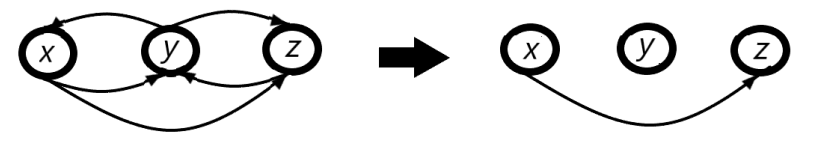
\includegraphics[width=0.5\textwidth]{images/25}}
\end{figure}

\par \textbf{Утверждение (задача 7.7):} квазитранзитивное отношение является ациклическим
\par $\blacktriangle$ Пусть это не так. Тогда существует некоторое конечное множество вершин $M_0$ являющееся циклом, т.е. $m_0 \prec m_1 \prec ... \prec m_k \prec m_0$. Тогда по транзитивности получаем $m_0 \prec m_k$, но $m_k \prec m_0$ - противоречие определению $\prec \quad \Rightarrow$ отношение ациклическое $\blacksquare$ 
\par \textbf{Задача 7.8:} Придумайте ациклическое отношение, не являющееся квазитранзитивным. Может ли такое отношение быть полным?
\par \textbf{Решение:} Например, $\{(a, b), (b, c)\}\subset\{a, b, c\}^2$ (думаю, комментарии излишни). 
\par Пусть есть полное ациклическое не квазитранзитивное отношение $\preccurlyeq$ над $A$, тогда $\exists x, y, z\in A$, такие что $x\prec y \wedge y\prec z \wedge \neg (x\prec z)$ (отрицание определения квазитранзитивности). Так как отношение полное, то $z\prec x$, но тогда во множестве $A' = \{x, y, z\}$ $\forall a\in A'\; \exists b\in A': a\prec b$ - противоречие $\Rightarrow$ такое отношение не может быть полным
 $\blacksquare$\\